\chapter{Initial exploration}
\label{cha:1}
In this chapter an initial exploration of the problem is perfomed. The direct multiple shooting approach will be solved using a general nonlinear solver. For a couple small test problems the novel algorithm will be compared to the industry standard backpropagation algorithm

\section{Direct Multiple Shooting Approach}
The optimal control problem (OCP) of training a neural network in \ref{ocp-eq} that is at the core of this thesis is repeated here again:

\begin{equation}
	\begin{aligned}
	& \underset{W}{\text{minimize}}
	& & \sum\limits_{j=0}^{n}||\sigma_L(W_Lz_L) - y_j||^2_2 \\
	& \text{subject to}
	& & z_{1,j} = \sigma_0(W_0,x_j), &j = 1,\ldots,n \\
	& & & z_{k+1,j} = \sigma_k(W_kz_{k,j}), &k = 1,\ldots,L-1,j = 1,\ldots,n
	\end{aligned}
	\label{ocp-eq2}
\end{equation}

This is a nonlinear program with nonlinear equality constraints. It is possible to eliminate the states $z_k$ using the dynamics, giving rise to an unconstrained nonlinear program as follows:

\begin{equation}
	\begin{aligned}
	& \underset{W}{\text{minimize}}
	& & \sum\limits_{j=0}^{n}||f_W(x_j) - y_j||^2_2 \\
	\end{aligned}
\end{equation}

where $f_W$ is the neural network as a function as in \ref{nnfnc}. Solving this problem would be the single shooting approach. One can find the gradient of this function using dynamic programming techniques, leading again to the backpropagation algorithm. A full derivation of the backpropagation algorithm using control theory can be found in Mizutani et al. \cite{mizutani2000} and Dreyfus et al. \cite{dreyfus1990}

This thesis instead tries to solve equation \label{ocp-eq2} directly, which corresponds to a multiple shooting approach.

\section{Test setup}
Before writing a custom solver, the problem is explored using a general nonlinear program(NLP) solver. For this task the \texttt{fmincon} method implemented in MATLAB is used together with the YALMIP optimization library. This method implements a interior point algorithm for solving constrained NLPs. 

For comparison against the standard backpropagation the neural network toolbox of MATLAB is used. The default training algorithm in this toolbox is \texttt{trainlm} which implements a Levenberg-Marquardt backpropagation algorithm. However this method is too well suited for the simple curve fitting problem the next sections use for testing. As figure \ref{trainlm} shows, this algorithm finds a perfect fitting curve almost every time. For this reason \texttt{traingd} is used instead, which is a standard Gradient Descent(GD) backpropagation algorithm. GD based algorithms such as ADAM are some of the most used algorithms in practice because of their simplicity and low cost per epoch.[REF] In contrast to \texttt{trainlm} this method will often settle in a "bad" local minimum and will not reach the same performance.

The test case used in this chapter is a regression problem to fit a neural network to the following sine function:

\begin{equation}
y_j = -.8\sin(x_j) + \mathcal N(0,\delta), x \in [0,1], j = 1..N
\label{sin}
\end{equation}

where $\delta=0.1$ adds noise, and $N$ is the number of datapoints. The input-output pairs $(x_j,y_j)$ are split into a training set of size $\frac{4}{5}N$ and a test set of size $\frac{1}{5}N$. Figure \ref{trainlm} plots this function and shows the output of a network which has been fit using \texttt{trainlm}. This is also a clear example of overfitting.

This test problem, as well as the test problem used in chapter 3, \ref{}, come from the course on neural networks given at KU Leuven \cite{}. [version numbers, hardware specs]

\begin{figure}
	\centering
         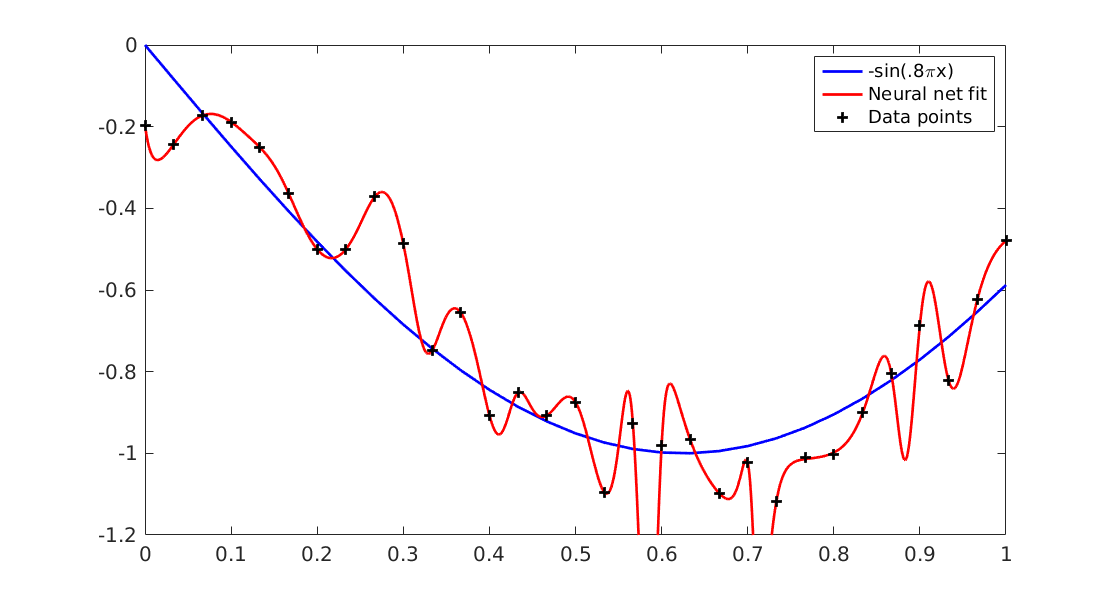
\includegraphics[width=\textwidth]{trainlm}
         \caption{Test function approximated with \texttt{trainlm} training algorithm. The data has been overfitted.}
         \label{trainlm}
\end{figure}

\section{Hyperbolic tangent activation function}
In a first experiment a small fully connected feedforward neural network is constructed with 2 hidden layers with each layer containing 3 nodes with a hyperbolic tangent activation function: $\tanh(x) = \frac{e^x-e^{-x}}{e^x+e^{-x}}$. This activation function is smooth and works well for small networks and for curve fitting. 

This network is fitted to the data described in the previous section using both algorithms. For the convergence of the multiple shooting method it is important that the initial point is feasible, therefore the state variables $z_k$ will be initiatialized by simulating the network once using random initialization for the weights.

Figure \ref{compalg} shows the result of a good training run for each algorithm. Figure \ref{gdtrain} and \ref{fmintrain} show the training performance per epoch. The gradient descent algorithm trains for many more iterations, but each iterate is much cheaper. Both algorithms stop progressing after a while, indicating a local minimum has been reached. The prediction of the network after training is plotted in \ref{gdfit} and \ref{fminfit}.

\begin{figure}
     \centering
     \begin{subfigure}[b]{0.4\textwidth}
         \centering
         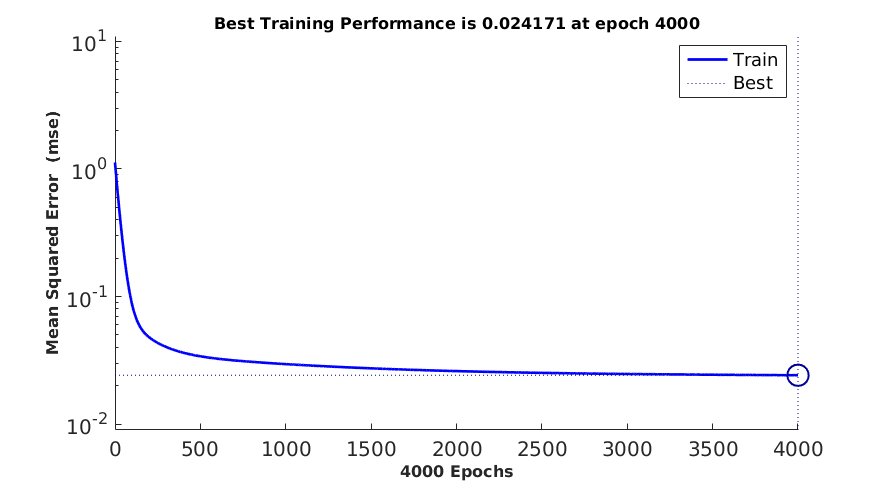
\includegraphics[width=\textwidth]{gdtrain}
         \caption{Training performance of Gradient Descent}
         \label{gdtrain}
     \end{subfigure}
     \begin{subfigure}[b]{0.4\textwidth}
         \centering
         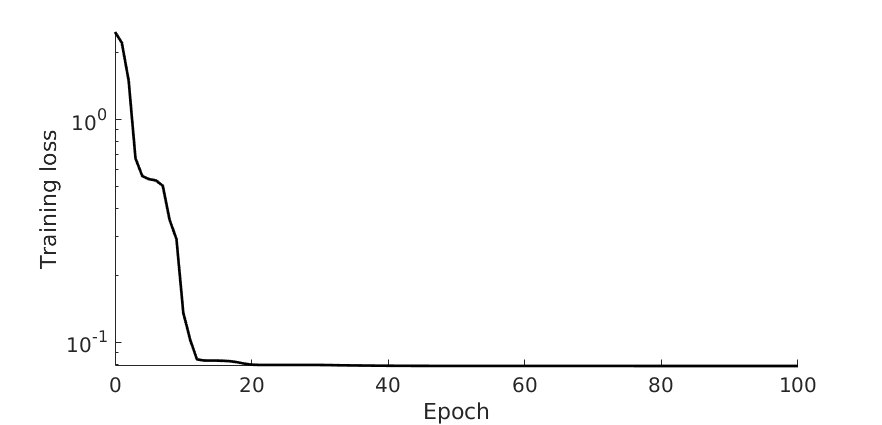
\includegraphics[width=\textwidth]{fmintrain}
         \caption{Training performance of Multiple Shooting}
         \label{fmintrain}
     \end{subfigure}
     \begin{subfigure}[b]{0.45\textwidth}
         \centering
         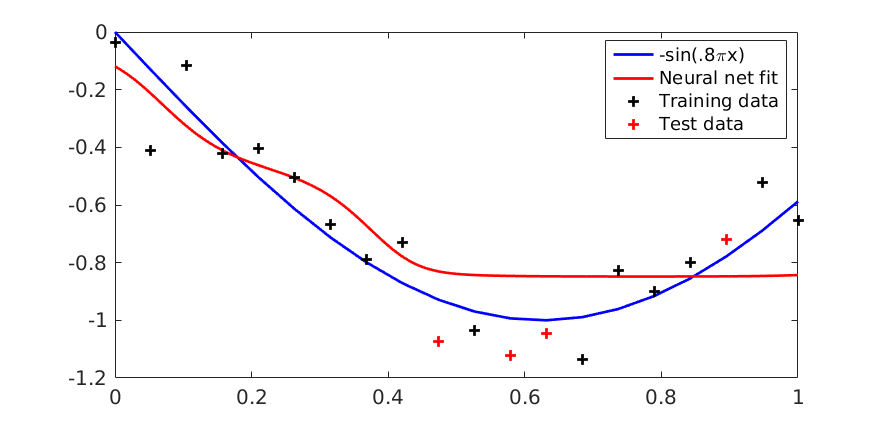
\includegraphics[width=\textwidth]{gdfit}
         \caption{Neural network fit with Gradient Descent}
         \label{gdfit}
     \end{subfigure}
     \begin{subfigure}[b]{0.45\textwidth}
         \centering
         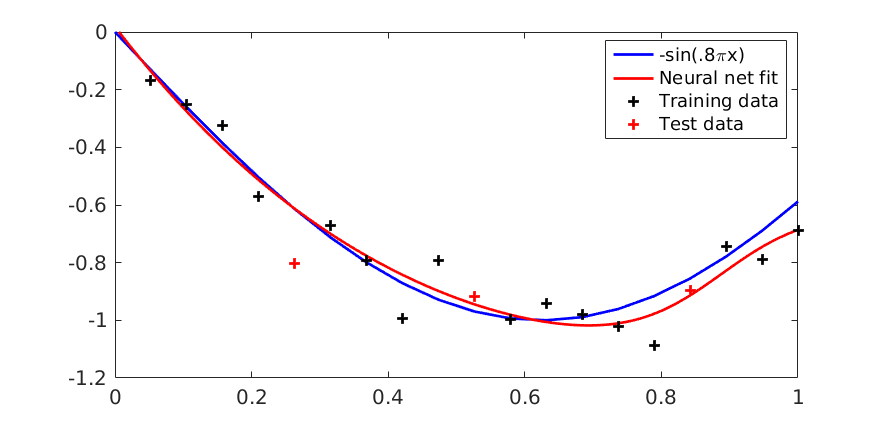
\includegraphics[width=\textwidth]{fminfit}
         \caption{Neural network fit with Multiple Shooting}
         \label{fminfit}
     \end{subfigure}
    \caption{Comparing algorithm performance for regression problem}
    \label{compalg}
\end{figure}

To quantify the difference in performance, each algorithm is run for 20 training runs. In each run both algorithms start with the same data and same initial weights. The weight initialization function is \texttt{initnw} which implements Nguyen-Widrow weight initialization. GD and MS are run for 2000 epochs and 40 epochs respectively, values which are chosen based on when each algorithm usually stops improving. The results are shown in table \ref{tab:tanh}.

\begin{table}
	\centering
	\begin{tabular}{r | c c c c c}
		Algorithm & \small best tr MSE & \small avg tr MSE & \small avg test MSE & \small avg run time \\ \hline
		Gradient Descent & 0.0108 & 0.0299 & 0.0605 & 1.577s \\
		Multiple Shooting & 0.0537 & 0.2350 & 0.2724 & 23.82s \\
	\end{tabular}
	\caption{Result of 20 training runs for each algorithm for $tanh$ activation function. Average MSE values are calculated over those runs which converged.}
	\label{tab:tanh}
\end{table}

Using \texttt{fmincon}, MS only converges 6 out of 20 times, while GD always converges. GD also has much better average performance and runs much quicker. However, at its best, MS can at least show similar performance to GD. The GD algorithm runs on GPU while the MS algorithm runs on CPU, so faster runs should be expected.

\section{Rectified linear unit}
In this section the same experiment as last time is run, but with a different network architecture. Again a network of two layers is used, but with 8 neurons in each layer, and using a ReLU activation function. 

For the multiple shooting approach the RELU activation function will have to be reformulated, in order to have smooth constraints. The ReLU function can be transformed as follows:

\begin{gather*}
   x_{k+1}^j = \max(W_kx_k^j,0) \\
   \Updownarrow \\
   x_{k+1}^j = -\min(-W_kx_k^j,0) \\
   \Updownarrow \\
   \min(x_{k+1}^j-W_kx_k^j) = 0 \\
   \Updownarrow \\
   (x_{k+1}^j-W_kx_k^j)^\top x_{k+1}^j = 0,\\
   x_{k+1}^j\geq 0,x_{k+1}^j-W_kx_k^j\geq 0
\end{gather*}


Table \ref{tab:relu} shows the results after 20 training runs, under the same conditions as the previous section. In this case MS converged 16/20 times, while GD still always converges. GD still runs at the same speed as the previous test despite the larger nextwork, while the run time for MS has significantly increased. 
   
   
\begin{table}
	\centering
	\begin{tabular}{r | c c c c c}
		Algorithm & \small best tr MSE & \small avg tr MSE & \small avg test MSE & \small avg run time \\ \hline
		Gradient Descent & 0.0041 & 0.0274 & 0.0489 & 1.480s \\
		Multiple Shooting & 0.0348 & 0.2111 & 0.2696 & 115.8s \\
	\end{tabular}
	\caption{Result of 20 training runs for each algorithm for ReLU activation function. Average MSE values are calculated over those runs which converged.}
	\label{tab:relu}
\end{table}


\section{Conclusion}
The MS algorithm did not outperform the GD in any way in either of the tests. However this chapter has demonstrated that it is feasible to train a network in this manner. Good solutions are possible using this method. The main issue is that \texttt{fmincon} is a very general method, and not well suited to this specific problem. For this reason the next chapter will explore the Augmented Langrangian Method (ALM), a common algorithmic framework for solving constrained NLPs.




%%% Local Variables: 
%%% mode: latex
%%% TeX-master: "thesis"
%%% End: 
